\chapter{Contour integration}
\section{Definitions}
\lecture{1}{13/1}

In contour integration, we study 
\[ \int_{\gamma} f(z) \, dz \]
where $f: U \to \C$ ($U \subset \C$ open) and 
$\gamma$ is a \emph{contour} (a special type of curve). 

Before we move onto this, we will start by considering complex valued functions
of \emph{real} variables.
If $f: [a, b] \to \C$ is continuous, with $f = u + iv$ ($u, v: [a, b] \to \R$) then
\[ \int_a^b f(z) \, dz = \int_a^b u(t) \, dt + i \int_a^b v(t) \, dt.\]

\begin{example}
    \[ \int_0^1 (t + it) \, dt =
        \int_0^1 t \, dt + i \int_0^1 t \, dt =
        \left(\frac12t^2\right)^1_0 + i\left(\frac12t^2\right)^1_0 =
        \frac12 + i\frac12.
    \]
\end{example}

\begin{lemma}[]
    Let $f, g: [a, b] \to \C$ be continuous and $c \in \C$. Then
    \begin{enumerate}
        \item 
            \[ \int_a^b(f(t) + g(t)) \, dt = \int_a^b f(t) \, dt + \int_a^b g(t) \, dt; \]

        \item
            \[ \int_a^b cf(t) \, dt = c \int_a^b f(t) \, dt. \]
    \end{enumerate}
\end{lemma}

\begin{proof}
    Easy exercise.
\end{proof}

\begin{remark}
    Recall that a curve is a continuous function $\gamma: [a, b] \to \C$.
    A curve is \emph{smooth} (or $C^1$) if it is \emph{continuously differentiable}.
\end{remark}

\begin{figure}
    \centering
    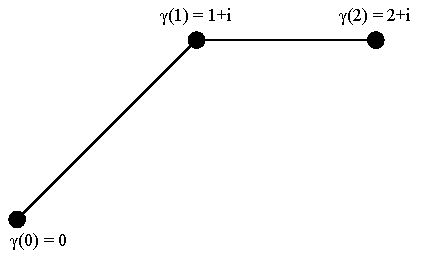
\includegraphics[width=0.6\linewidth]{images/continuous-curve-ex.pdf}
    \caption{A continuous (but not differentiable) curve.}%
    \label{fig:continuous-curve-ex}
\end{figure}

\begin{example}
    \begin{enumerate}
        \item Let $r > 0$ and $\gamma(t) = re^{it}$ for $t \in [0, 2\pi]$.
            This defines a curve that is a circle of center $0$ and radius $r$ 
            which is traversed anticlockwise.

        \item Now the same as before but let $\gamma(t) = re^{-it}$. 
            This defines the same circle as before but is traversed clockwise.

        \item Let the function $\gamma: [0, 2] \to \C$ be defined as
            \[
                \gamma(t) =
                \begin{cases}
                    t + it & t \in [0, 1] \\
                    t + i  & t \in [1, 2].
                \end{cases}
            \]
    \end{enumerate}
    This curve is shown in Figure \ref{fig:continuous-curve-ex}.
    $\gamma$ is continuous; however, it is not $C^1$ as $\gamma'(t)$ is not defined
    for $t = 1$.
\end{example}

\begin{definition}[Contour integral]
    Let $U \subset \C$ be open, 
    $f: U \to \C$ be continuously differentiable, 
    and $\gamma: [a, b] \to U$ be a $C^1$ curve.
    Then
    \[ \int_\gamma f(z) \, dz = \int_a^b f(\gamma(t)) \gamma'(t) \, dt.\]
\end{definition}

\begin{remark}
    $\gamma'(t)$ exists as $\gamma$ is continuous differentiable ($C^1$).
    The integrand is a complex-valued function of a \emph{real variable}.
\end{remark}

\begin{proposition}[Basic properties of contour integrals]
    Let $f, g: U \to \C$ ($U \subset \C$ open), $\gamma: [a, b] \to U$ be a $C^1$ curve,
    and $c \in \C$. Then the following hold.
    \begin{enumerate}
        \item 
            \[ \int_\gamma(f(z) + g(z))\,dz = \int_\gamma f(z) \, dz + \int_\gamma g(z) \, dz. \]

        \item 
            \[ \int_\gamma cf(z) \, dz = c \int_\gamma f(z) \, dz. \]

        \item We define $(-\gamma): [-b, -a] \to \C$ by $(-\gamma)(t) = \gamma(-t)$. Then
            \[ \int_{(-\gamma)} f(z) \, dz = - \int_\gamma f(z) \, dz. \]
    \end{enumerate}
\end{proposition}

\begin{example}
    Let $r > 0$ and $\gamma: [0, 2\pi] \to \C$ be defined by
    \[ \gamma(t) = re^{it}. \]
    Calculate
    \[ \int_\gamma \, dz. \]
\end{example}

\begin{solution}
    Here $f(z) = 1$.
    \begin{align*}
        \int_\gamma \, dz
        &= \int_\gamma 1 \, dz \\
        &= \int_0^{2\pi} 1 \cdot rie^{it} \, dt \\
        &= ri \int_0^{2\pi} (\cos{t} + i\sin{t}) \, dt = 0.
    \end{align*}
\end{solution}

\begin{example}
    Let $\gamma(t) = 2e^{it}$
    where $\gamma: \left[-\frac12, \frac12\right] \to \C$.
    Integrate
    \[ \int_\gamma \overline z \, dz. \]
\end{example}

\begin{solution}
    Here $f(z) = \overline z$.
    Then $f(\gamma(t)) = \overline{2e^{it}} = 2e^{-it}$.
    So
    \begin{align*}
        \int_\gamma \overline z \, dz 
        &= \int_{-\frac{\pi}2}^{\frac{\pi}2} \left(2e^{-it}\right) \left(2ie^{it}\right) \, dt \\
        &= 4i \int_{-\frac{\pi}2}^{-\frac{\pi}2} \, dt = 4\pi i.
    \end{align*}
\end{solution}

\begin{lemma}[Reparametrisation of curves]
    Let $U \subset \C$ be open,
    $f: U \to \C$ be continuous, and
    $\gamma: [a, b] \to U$ be a $C^1$ curve.
    If $\phi: [a', b'] \to [a, b]$ with 
    $\phi(a') = a$ and $\phi(b') = b$ is continuously differentiable and 
    \[ \delta: [a', b'] \to \C, \qquad \delta = \gamma \circ \phi \]
    then we have
    \[ \int_\gamma f(z) \, dz = \int_\delta f(z) \, dz. \]
\end{lemma}


